\documentclass[english]{ufsc-thesis-rn46-2019}

\usepackage[utf8]{inputenc} % UTF-8
\usepackage{lipsum} % Gerador de texto
\usepackage{pdfpages} % Inclui PDF externo (ficha catalográfica)


% Preâmbulo
\titulo{Template \LaTeX~ seguindo a RN 46/2019/CPG da UFSC}
\autor{Fulano da Silva}
% Importante! Para documentos em inglês, não use today, digite a data em
% pt_BR, como deve aparecer na folha de certificação.
\data{1 de Agosto de 2019}
\instituicao{Universidade Federal de Santa Catarina}
\programa{Programa de Pós-Graduação em Ciências da Computação}
\tese % ou \dissertacao
\local{Florianópolis} % Apenas cidade! Sem estado
\titulode{Doutor em Ciência da Computação}
\orientador{Prof. Dr. Ben Trovato}
\coorientador{Prof. Dr. Lars Thørväld}
\centro{Centro Tecnológico -- CTC}

% Membros da banca e coordenador
% As regras da BU agora exigem que Dr. apareça depois do nome
\membrobanca{Prof. Valerie Béranger, Dr.}{Universidade Federal de Santa Catarina}
\membrobanca{Prof. Aparna Patel, Dr.}{Universidade Federal de Santa Catarina}
\membrobanca{Prof. Huifen Chan, Dr.}{Universidade Federal de Santa Catarina}
% Atenção! o template da BU e o documento que apresenta as regras continua
% usando Dr antes do nome para Orientador e Coordenador!
\coordenador{Prof. Dr. Charles Palmer, Dr.}


\begin{document}

% Inicia parte pré-textual do documento capa, folha de rosto, folha de
% aprovação, aprovação, resumo, lista de tabelas, lista de figuras, etc.
\pretextual%
\imprimircapa%
\imprimirfolhaderosto*
\clearpage % força troca de página. Importante fazer isso antes do includepdf
% Ficha catalográfica deve ser gerado no site http://ficha.bu.ufsc.br/
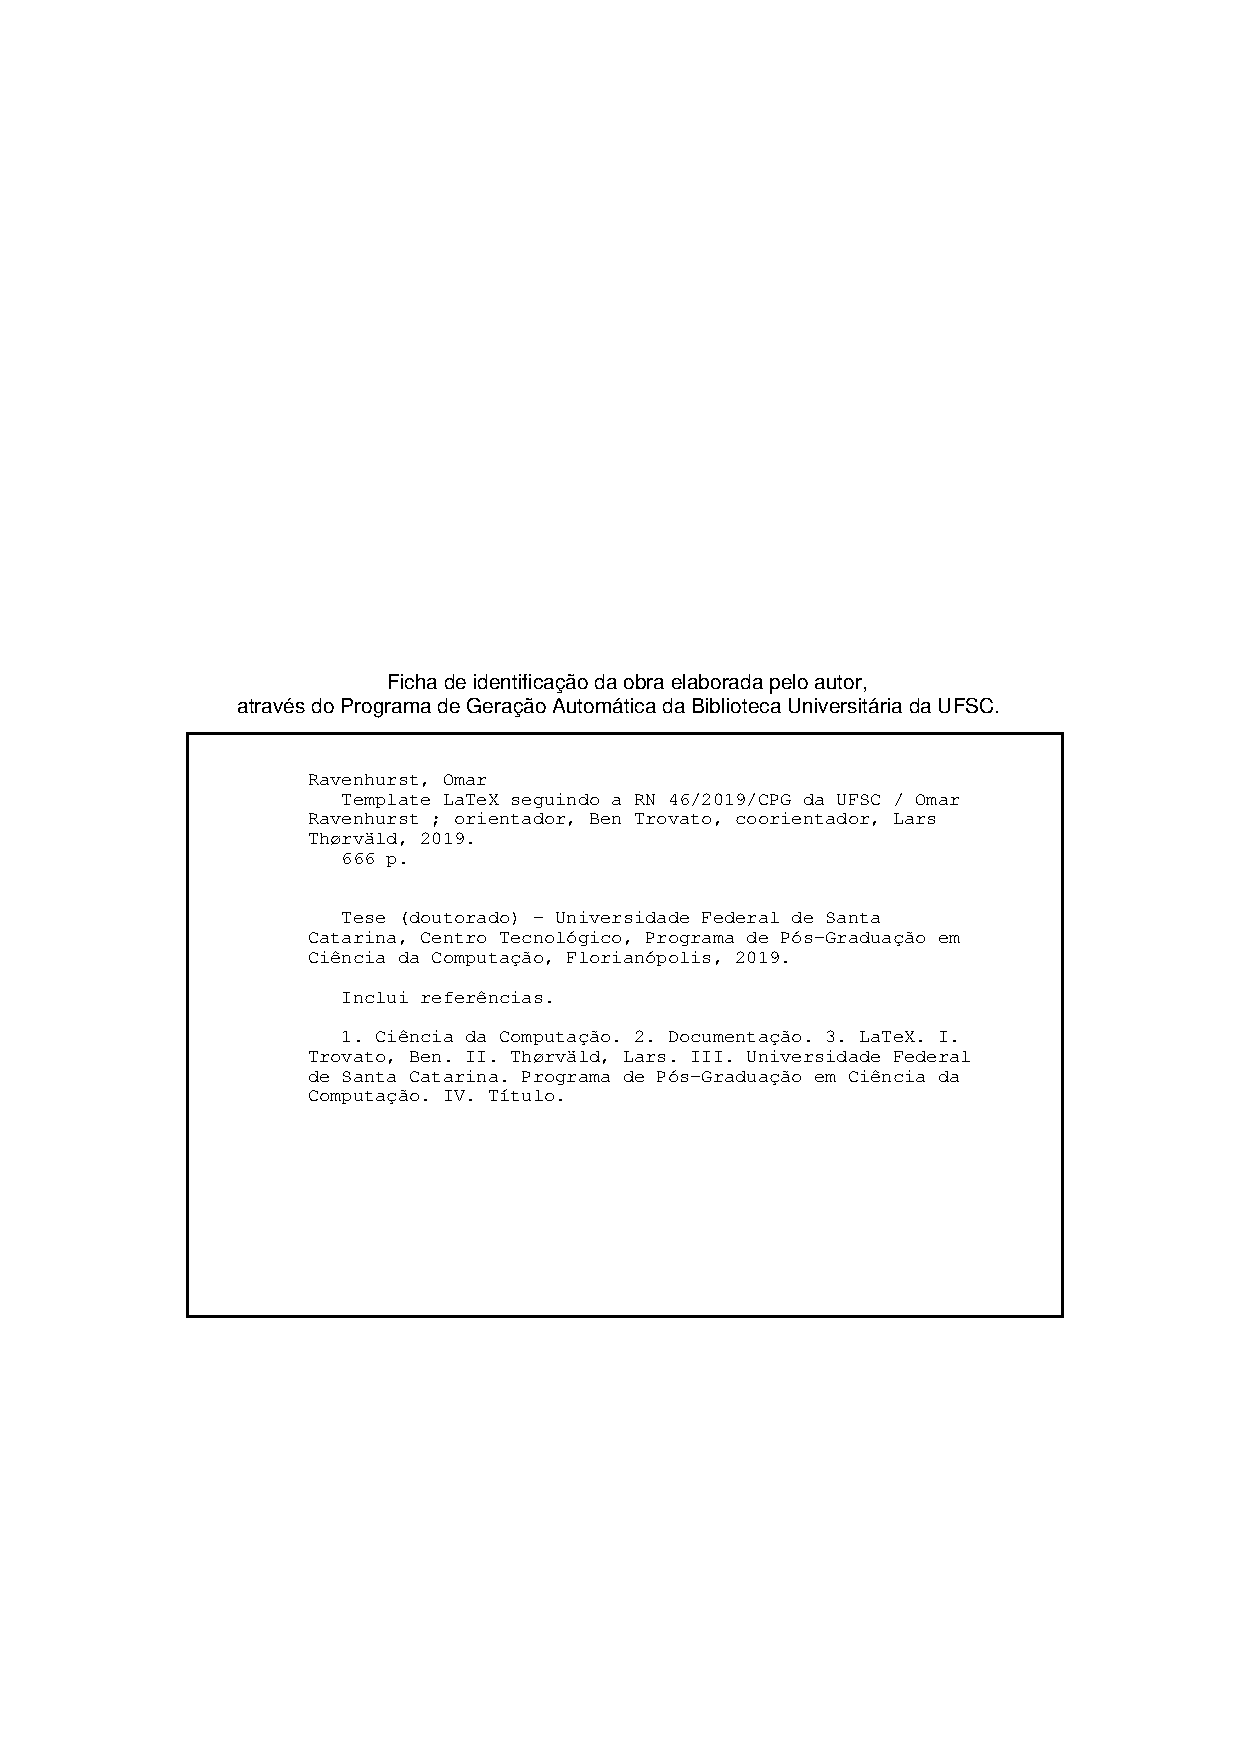
\includepdf{ficha.pdf}
\clearpage
\imprimirfolhadecertificacao
\listoffigures*
\cleardoublepage
\tableofcontents*%
\textual%

\chapter{Introduction}

This is the introduction. Lorem ipsum dolor sit amet, consectetur adipiscing elit, sed do eiusmod tempor incididunt ut labore et dolore magna aliqua. Ut enim ad minim veniam, quis nostrud exercitation ullamco laboris nisi ut aliquip ex ea commodo consequat. Duis aute irure dolor in reprehenderit in voluptate velit esse cillum dolore eu fugiat nulla pariatur. Excepteur sint occaecat cupidatat non proident, sunt in culpa qui officia deserunt mollit anim id est laborum.

Meaningless and wordy sentence with a reference to a seminal article in the hope of averting attention to the lack of content while at the same time borrowing some credibility \cite{turing1937computable}. This harmless sentence tests a nominal reference to \citeonline{dijkstra1968go}.

\begin{itemize}
\item \autoref{ch:bg}
\item \autoref{sec:stuff}
\item \autoref{sec:more}
\item \autoref{sec:yet-more}
\end{itemize}

\lipsum[1]

\chapter{Background}
\label{ch:bg}

\lipsum[1]

\section{Some stuff}
\label{sec:stuff}

\lipsum[1]

\section{Some other stuff}

Atenção! O template da BU deixa figuras e tabelas alinhadas à esquerda. No entanto, o tutorial de Word disponibilizado pela BU diz que Legendas e captions devem respeitar o ``alinhamento da ilustração'' (e apresenta uma ilustração alinhada a esquerda). O tutorial explicando a ABNT mostra uma figura centralizada com legendas alinhadas a esquerda e com recuo até o começo da figura. O autor do .cls se exime de qualquer culpa. Alinhe aqui (com \textbackslash{}centering \textbackslash{}flushright ou \textbackslash{}flushleft) como mandar o seu coração.

\begin{figure}[tb]
  \centering
  \caption{\footnotesize A caption text.}
  \label{fig:f}
  %\lipsum[1]

  <Fig here>
  \captionsource{The author.}
\end{figure}


\subsection{Some more stuff}
\label{sec:more}

\lipsum[1] \footnote{Some footnote}
\footnote{Some Large footnote: \lipsum[4]}

\subsubsection{Yet more stuff}
\label{sec:yet-more}

\lipsum[1]

\subsubsubsection{Yet another more stuff}
\label{sec:yet-another}

\lipsum[1]

\postextual
\bibliography{example}

\end{document}
